\documentclass{standalone}
\usepackage{tikz}
\usetikzlibrary{positioning, arrows.meta, shapes.geometric, fit, calc}

\begin{document}
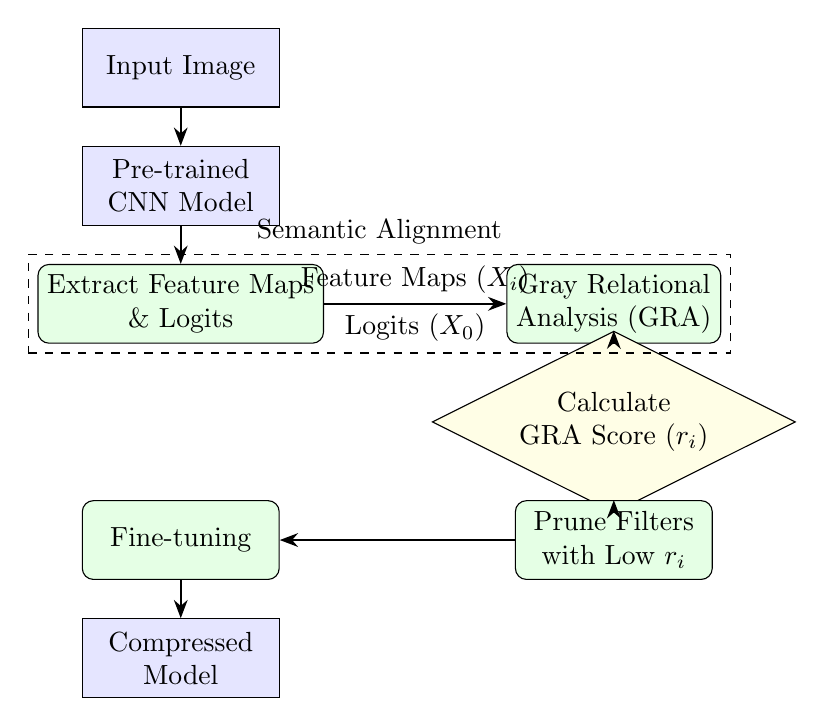
\begin{tikzpicture}[
    node distance=1.5cm,
    layer/.style={draw, rectangle, minimum width=2.5cm, minimum height=1cm, align=center, fill=blue!10},
    process/.style={draw, rectangle, rounded corners, minimum width=2.5cm, minimum height=1cm, align=center, fill=green!10},
    decision/.style={draw, diamond, aspect=2, minimum width=2.5cm, align=center, fill=yellow!10},
    arrow/.style={->, >=Stealth, thick}
]

% Nodes
\node (input) [layer] {Input Image};
\node (conv) [layer, below of=input] {Pre-trained\\CNN Model};
\node (activations) [process, below of=conv] {Extract Feature Maps\\\& Logits};

\node (gra) [process, right of=activations, xshift=4cm] {Gray Relational\\Analysis (GRA)};
\node (score) [decision, below of=gra] {Calculate\\GRA Score ($r_i$)};

\node (prune) [process, below of=score] {Prune Filters\\with Low $r_i$};
\node (finetune) [process, left of=prune, xshift=-4cm] {Fine-tuning};
\node (output) [layer, below of=finetune] {Compressed\\Model};

% Reference Sequence
\node (ref) [draw, dashed, fit=(activations) (gra), label=above:Semantic Alignment] {};

% Connections
\draw [arrow] (input) -- (conv);
\draw [arrow] (conv) -- (activations);
\draw [arrow] (activations) -- node[above] {Feature Maps ($X_i$)} node[below] {Logits ($X_0$)} (gra);
\draw [arrow] (gra) -- (score);
\draw [arrow] (score) -- (prune);
\draw [arrow] (prune) -- (finetune);
\draw [arrow] (finetune) -- (output);

% Feedback/Loop (optional)
%\draw [arrow] (finetune) -| (conv);

\end{tikzpicture}
\end{document}
